\documentclass[brazil,times]{abnt}
\usepackage[T1]{fontenc}
\usepackage[utf8]{inputenc}
\usepackage{url}
\usepackage{graphicx}
\usepackage[pdfborder={0 0 0}]{hyperref}
\usepackage{amssymb}
\usepackage{amsmath}
\usepackage[section]{placeins}
\usepackage{listingsutf8}
\makeatletter
\usepackage{babel}
\makeatother


\lstset{
	language=Octave,
	tabsize=2,
	inputencoding=utf8,
	basicstyle=\scriptsize,
	showspaces=false,
	showstringspaces=false,
	showtabs=false,
}

\begin{document}


\autor{Pedro Paulo Vezzá Campos}

\titulo{Métodos de Processamento de Imagens}

\comentario{Segundo exercício-programa apresentado para avaliação na disciplina
MAC0300, do curso de Bacharelado em Ciência da Computação, turma 45, da
Universidade de São Paulo, ministrada pelo professor Walter Figueiredo Mascarenhas.}

\instituicao{Departamento de Ciência da Computação \par Instituto de Matemática
e Estatística \par Universidade de São Paulo}

\local{São Paulo - SP, Brasil}

\data{\today}

\capa

\folhaderosto

\tableofcontents

\chapter{Introdução\label{cap:introducao}}
	Neste segundo exercício-programa de MAC0300 - Métodos Numéricos da Álgebra Linear foi pedido que implementássemos um programa que fosse capaz de aplicar diferentes métodos de processamento de imagens em tons de cinza. Neste relatório serão apresentados: Uma explicação e a implementação para cada um dos filtros pedidos no enunciado, testes realizados e, por fim, será feita apresentada uma conclusão sobre o EP.

%Explique suscintamente o processo utilizado na implementação de cada um dos filtros;

%Mostre, para cada um dos métodos solicitados, as imagens originais e as obtidas após o processamento.

%Descreva as vantagens e desvantagens de cada um dos métodos, tanto em relação ao desempenho computacional como em relação ao desempenho como filtro de imagem.
\chapter{Métodos de Processamento de Imagens}

	\section{Ajuste de Contraste - Equalização de Histograma}
		O processo de equalizar um histograma de uma imagem, isto é, tornar aproximadamente iguais as quantidades de cada um dos tons de cinza em uma imagem, é uma maneira computacionalmente simples de gerar imagens que tem, em geral, contrastes melhores que as originais.

		\subsection{Vantagens e desvantagens}
			Este método possui como vantagens o fato de geralmente produzir imagens com maior contraste. Isto acontece quando o primeiro plano e fundo da imagem são claros ou escuros. Após a equalização as diferenças nas tonalidades de ambos é mais exacerbada o que permite visualizar melhor diferentes detalhes. Por outro lado, imagens que já apresentam diferenças significativas nos tons de cinza não terão grandes ganhos após a equalização. Além disso, como este método não diferencia trechos da imagem, o método pode piorar a relação sinal/ruído da imagem já que ruidos antes pouco visíveis passam a ser mais evidenciados.
			O algoritmo para este método é bastante simples, como poderemos ver a seguir, e ainda a complexidade computacional é linear no tamanho da imagem e na quantidade de tons de cinza existentes, o que faz o método ser bastante utilizado na prática.
			
		\subsection{Implementação}
			A implementação deste método segue um algoritmo simples: Devemos primeiramente calcular o histograma da imagem original (\texttt{p}) e com ele produzir o histograma acumulado (\texttt{fda}). Com os valores mínimo e máximo de \texttt{fda} podemos utilizar a fórmula deduzida no enunciado do EP para $h_X (i)$ (No código, \texttt{h}) que produz um mapeamento entre um tom de cinza da imagem original e o tom de cinza na nova imagem equalizada. O último passo é realizar o mapeamento para determinar a nova imagem.


\begin{lstlisting}
function [imagem] = equalizar_histograma(imagem)
	m = rows(imagem);
	n = columns(imagem);
	p = zeros(256, 1);
	fda = zeros(256, 1);
	
	%Parte 1: Calculando o histograma
	for j = 1 : n
		for i = 1 : m
			p(imagem(i,j) + 1) += 1;
		endfor
	endfor
	
	%Parte 2: Calculando o histograma acumulado
	fda(1) = p(1);
	for i = 2 : 256
		fda(i) = fda(i - 1) + p(i);
	endfor
	
	fda_min = min(fda);
	fda_max = max(fda);
	
	%Parte 3: Calculando o mapeamento
	h = zeros(256,1);
	for i = 1 : 256
		h(i) = round((fda(i) - fda_min)/(m * n - fda_min) * 255);
	endfor
	
	%Parte 4: Realizando o mapeamento para gerar a nova imagem
	for j = 1 : n
		for i = 1 : m
			imagem(i, j) = h(imagem(i,j) + 1);
		endfor
	endfor
endfunction
\end{lstlisting}

		%Para o método de ajuste de contraste por equalização de histograma, apresente também os histogramas correspondentes às imagens original e processada.
		\subsection{Testes realizados}
			Para apresentar as mudanças no histograma e na aparência das imagens que o método causa são apresentadas dois exemplos de imagens antes e depois de aplicado o método tendo ao lado o respectivo histograma. Podemos ver como o histogramas novos são mais distribuídos ao longo do eixo das intensidades (Eixo x).
			
			\begin{table}[ht]
			\caption{Imagens antes e depois de aplicada a equalização e seus respectivos histogramas}
			\centering
			\begin{tabular}{|c|c|}
			\hline
			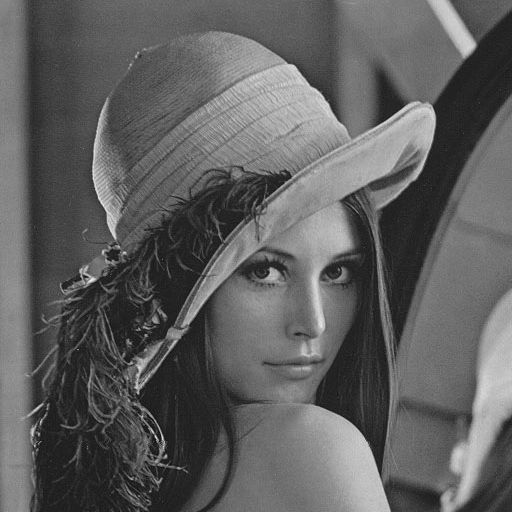
\includegraphics[scale=0.25]{imagens/lena.jpg}&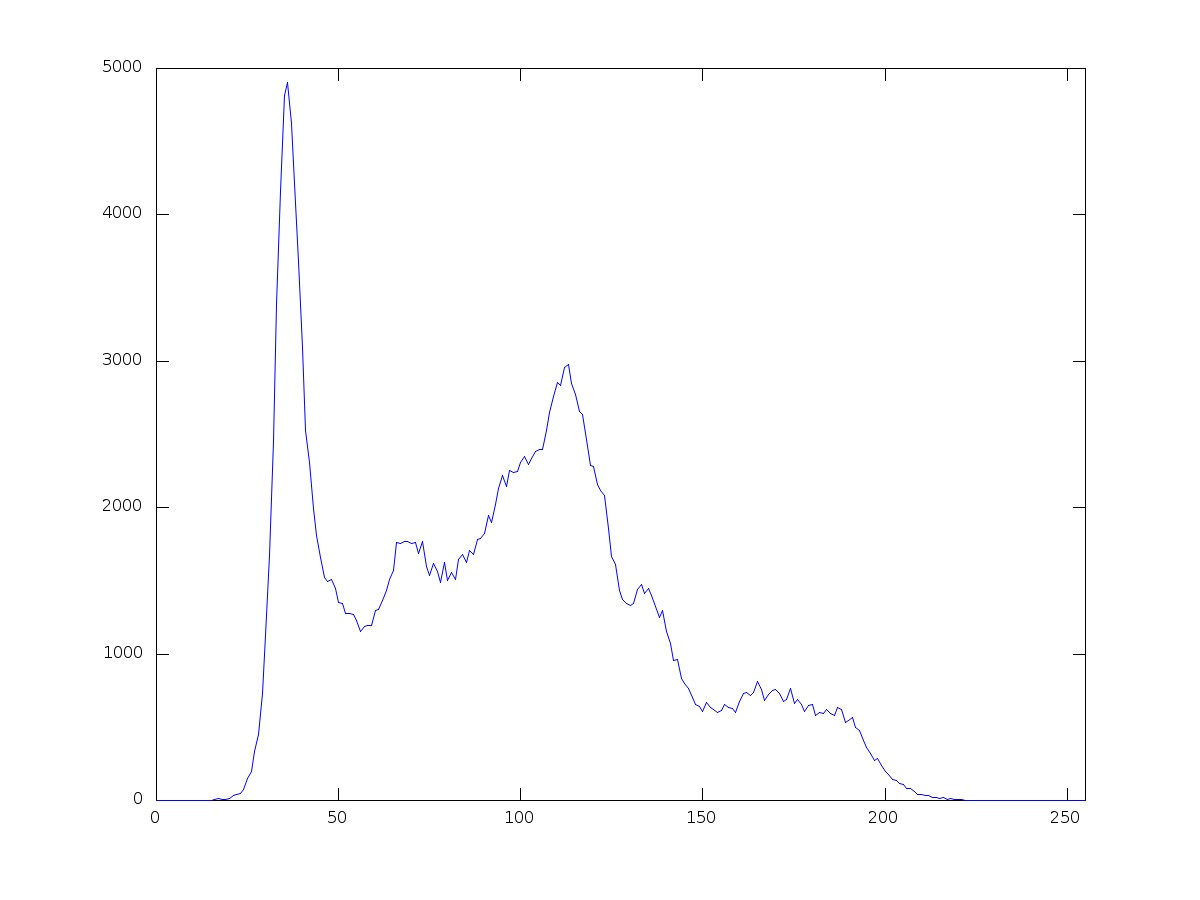
\includegraphics[scale=0.15]{imagens/lena-hist-original.jpg}\\
			\hline
			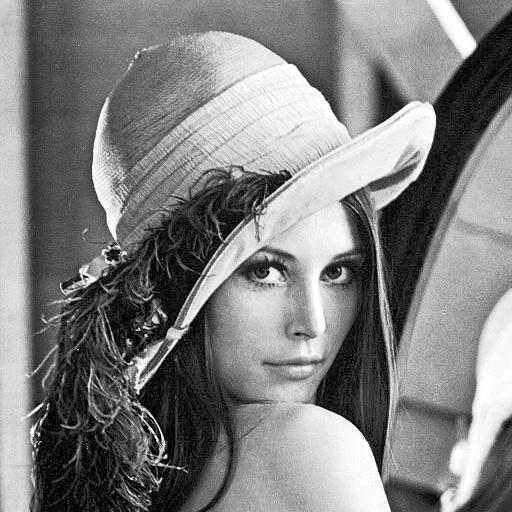
\includegraphics[scale=0.25]{imagens/lena-contrast.jpg}&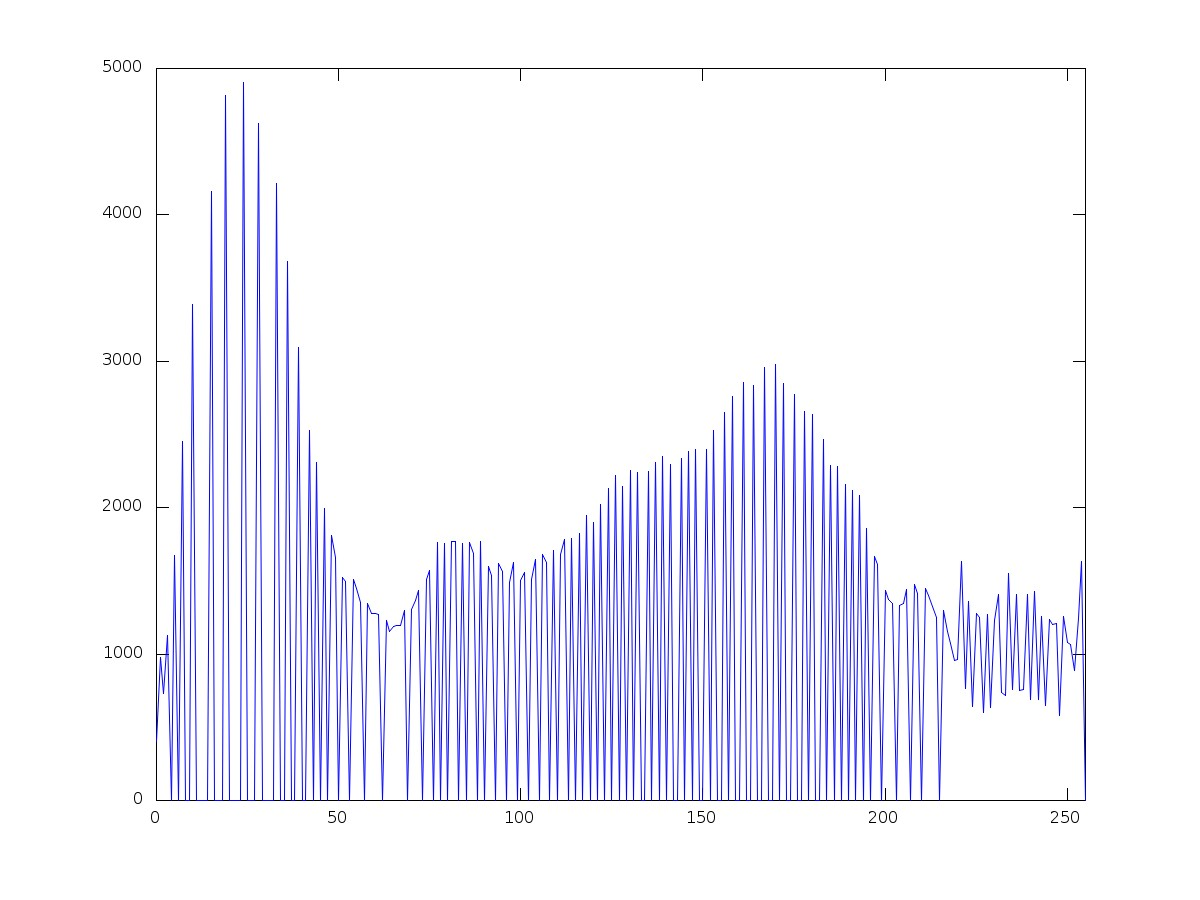
\includegraphics[scale=0.15]{imagens/lena-hist-novo.jpg}\\
			\hline
			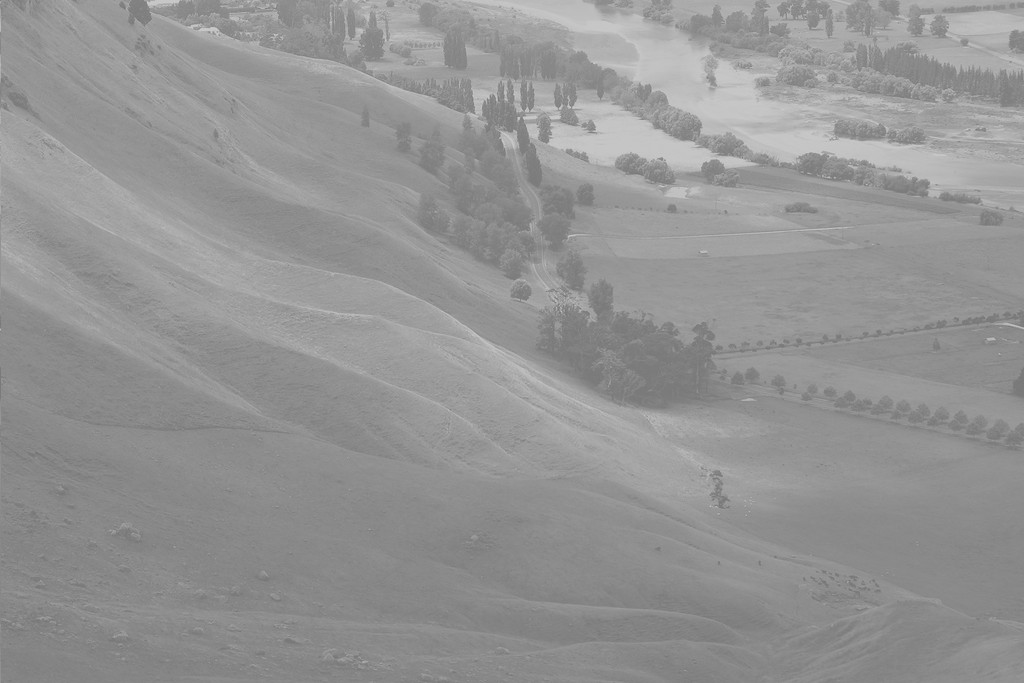
\includegraphics[scale=0.125]{imagens/hawkes.jpg}&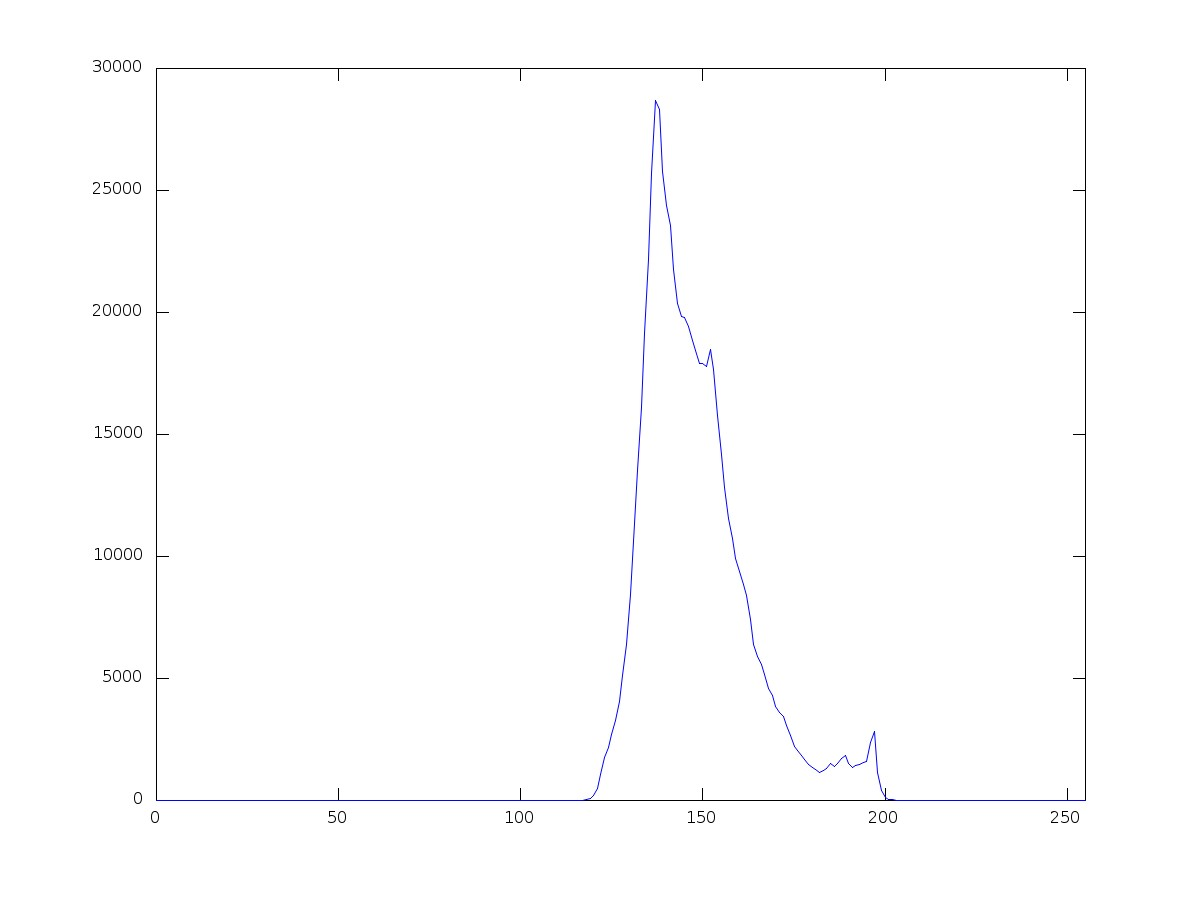
\includegraphics[scale=0.15]{imagens/hawkes-hist-original.jpg}\\
			\hline
			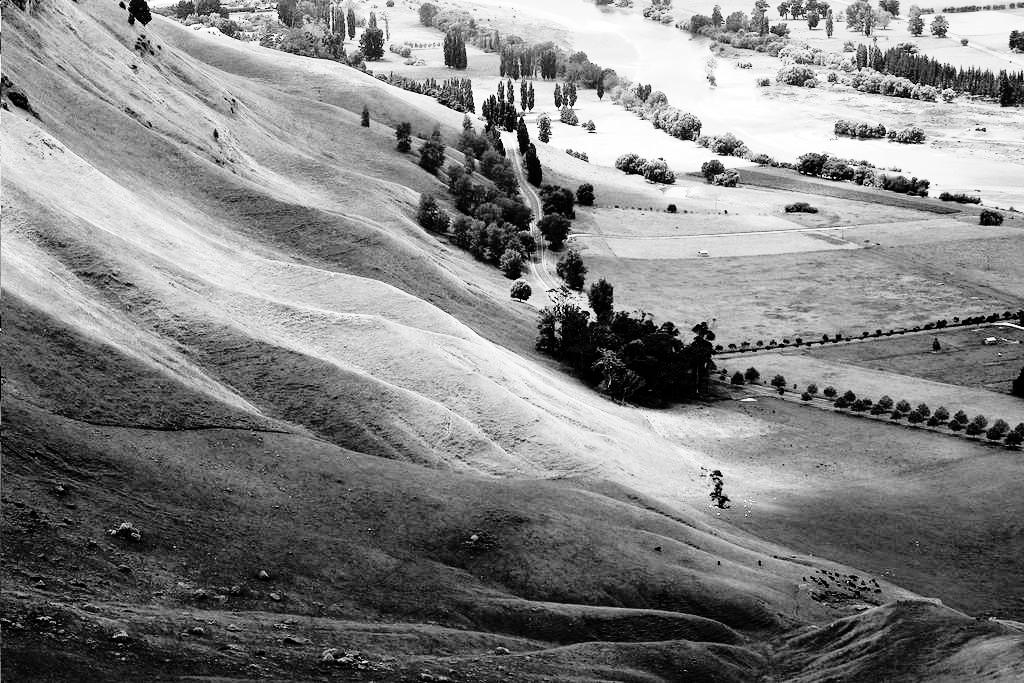
\includegraphics[scale=0.125]{imagens/hawkes-contrast.jpg}&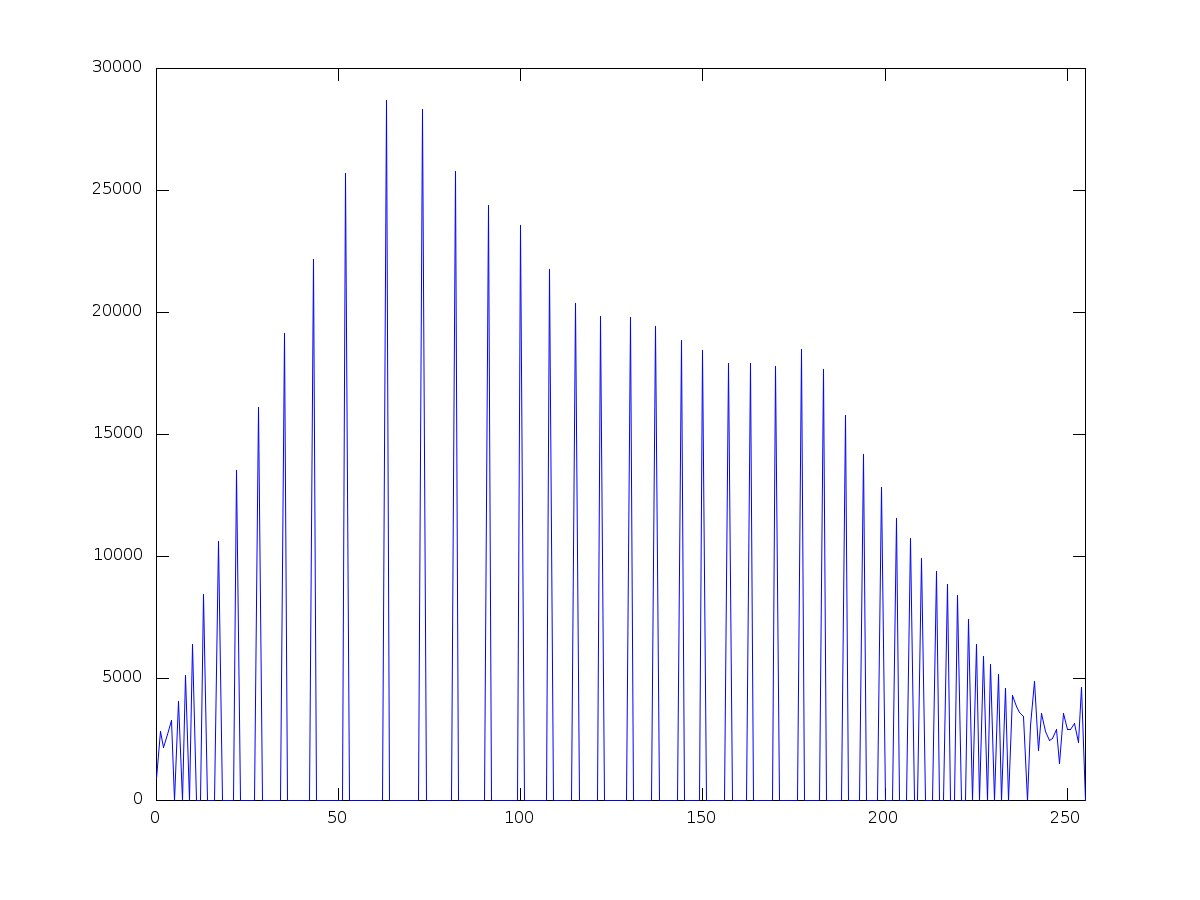
\includegraphics[scale=0.15]{imagens/hawkes-hist-novo.jpg}\\
			\hline
			\end{tabular}
			\label{tab:gt}
			\end{table}

	\section{Filtros por Convolução}
		Há uma classe de filtros aplicáveis em imagens, tais como os que serão apresentados a seguir, que são filtros lineares. Tais filtros tem a característica que um pixel após a filtragem é dado como uma combinação linear de seus vizinhos. Os coeficientes utilizados na combinação linear podem ser agrupados como uma matriz a qual se dá o nome de kernel. 
		O processo de aplicar a transformação a cada um dos pixels da imagem fazendo uso do kernel é chamada de convolução. Fazendo uso da fórmula fornecida no enunciado, foi implementada uma função de convolução que dada uma imagem e um kernel primeiramente cria uma borda de zeros em torno da imagem original e em seguida aplica a combinação. O efeito é que a imagem resultante tem o mesmo tamanho da original. A função assim, tem o mesmo comportamento de \texttt{filter2(kernel, imagem, "same")} da biblioteca padrão do Octave/Matlab.
		A vantagem de utilizar convoluções é que fica possível aplicar qualquer transformação linear de maneira bastante simples, bastando apenas definir o kernel correspondente. Transformações lineares são muito variadas, há as translações, suavizações, remoção de ruído, aumento de nitidez, detecções de borda, etc.
		A desvantagem de filtragens por convolução é que a quantidade de operações para a filtragem é maior que no caso anterior. Agora, para determinar cada pixel é necessário $n \times m$ operações de multiplicação onde $n$ e $m$ são as dimensões do kernel.
		
		\subsection{Implementação}
\begin{lstlisting}
function [C] = aplicar_convolucao(A, K)
    [m_A, n_A] = size(A);
    [m_K, n_K] = size(K);
	
	borda = zeros(m_A + 2, n_A + 2);
	borda(2 : m_A + 1, 2: n_A + 1) = A;
	A = borda;
	m_A += 2;
	n_A += 2;
	
    C = zeros(m_A - m_K + 1, n_A - n_K + 1);

    for i = 1 : m_A - 2
        for j = 1 : n_A - 2
            C(i, j) = sum(sum(A(i : i + m_K - 1, j : j + m_K - 1) .* K));
        endfor
    endfor
endfunction

\end{lstlisting}


	
	\section{Filtro de Suavização por Média Ponderada}
		Este filtro tem por objetivo a remoção de ruídos de uma imagem. Para isso, a abordagem que é adotada é o cálculo em que cada pixel da nova imagem passa a ser uma média ponderada de todos os seus pixels originais, atribuindo pesos distintos a cada um deles. Sua implementação pode ser feita através de filtragem por convolução. Nesta, damos um peso mais alto para o pixel original, um peso intermediário para os pixels acima, abaixo e aos lados e um peso menor para os da diagonal.
	
		\subsection{Vantagens e desvantagens}
			A vantagem principal deste método é a simplicidade. Como explicado anteriormente, uma filtragem por convolução utilizando um kernel da forma 
\[
 \frac{1}{16} \times 
 \begin{pmatrix}
  1 & 2 & 1 \\
  2 & 4 & 2 \\
  1 & 2 & 1 \\
 \end{pmatrix}
\]
		é suficiente para aplicar atingir o efeito desejado. A complexidade computacional é a mesma da filtragem por convolução. Por outro lado, como estamos realizando médias de pixels vizinhos há um probema de borramento (\emph{blurring}) da imagem inerente ao processo. Isso pode ser redizido através de técnicas para aumentar a nitidez. Uma destas técnicas será vista em seguida.
		
		\subsection{Implementação}
			Uma vez que foi implementada a filtragem por convolução, a implementação deste filtro torna-se trivial:
			
			\begin{lstlisting}
			function [final] = suavizar(imagem)
			    final = cast(aplicar_convolucao(imagem, [1 2 1; 2 4 2; 1 2 1]/16), "uint8");
			endfunction
			\end{lstlisting}
			
			Note que é necessário arredondar o resultado da convolução para que a imagem resultante possa ser gravada novamente.
		
		\subsection{Testes realizados}
			Nas imagens de teste podemos perceber como ruídos da forma "grãos claros e escuros" são reduzidos, porém, há um leve borramento do resultado, algo já esperado.
			
			\begin{table}[ht]
			\caption{Imagens antes e depois de aplicada a filtragem de suavização}
			\centering
			\begin{tabular}{|c|c|}
			\hline
			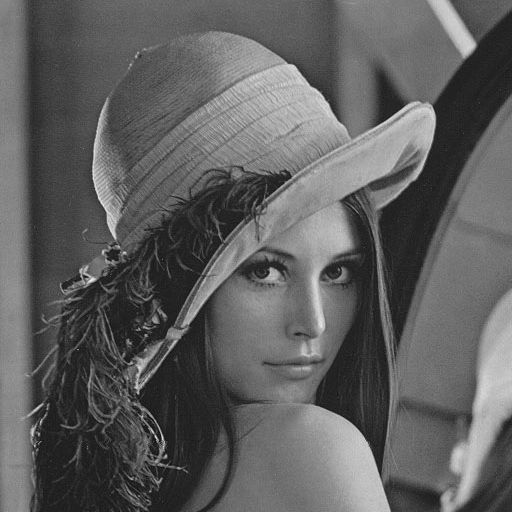
\includegraphics[scale=0.4]{imagens/lena.jpg}&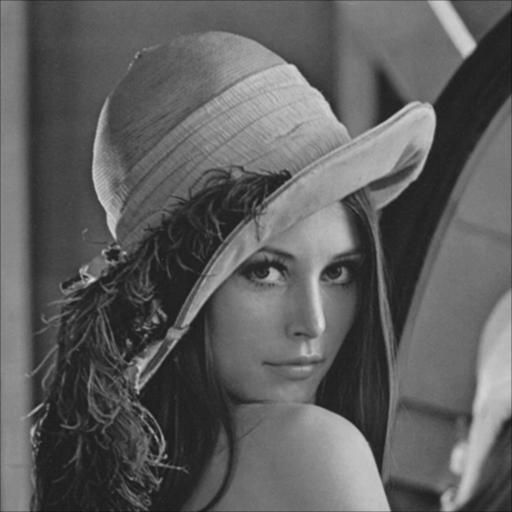
\includegraphics[scale=0.4]{imagens/lena-blur.jpg}\\
			\hline
			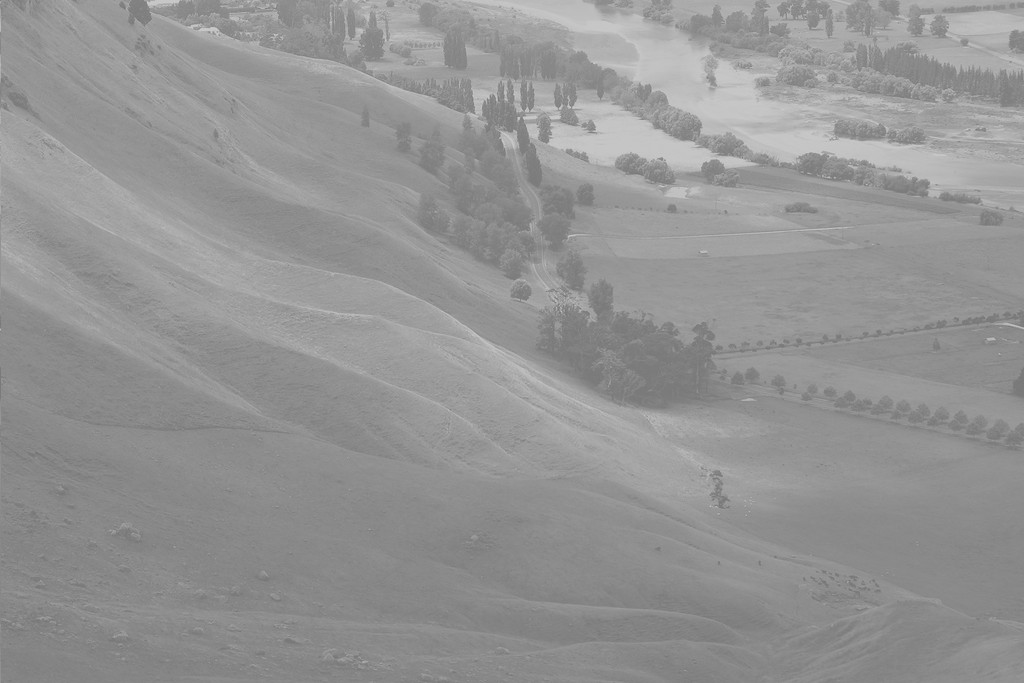
\includegraphics[scale=0.2]{imagens/hawkes.jpg}&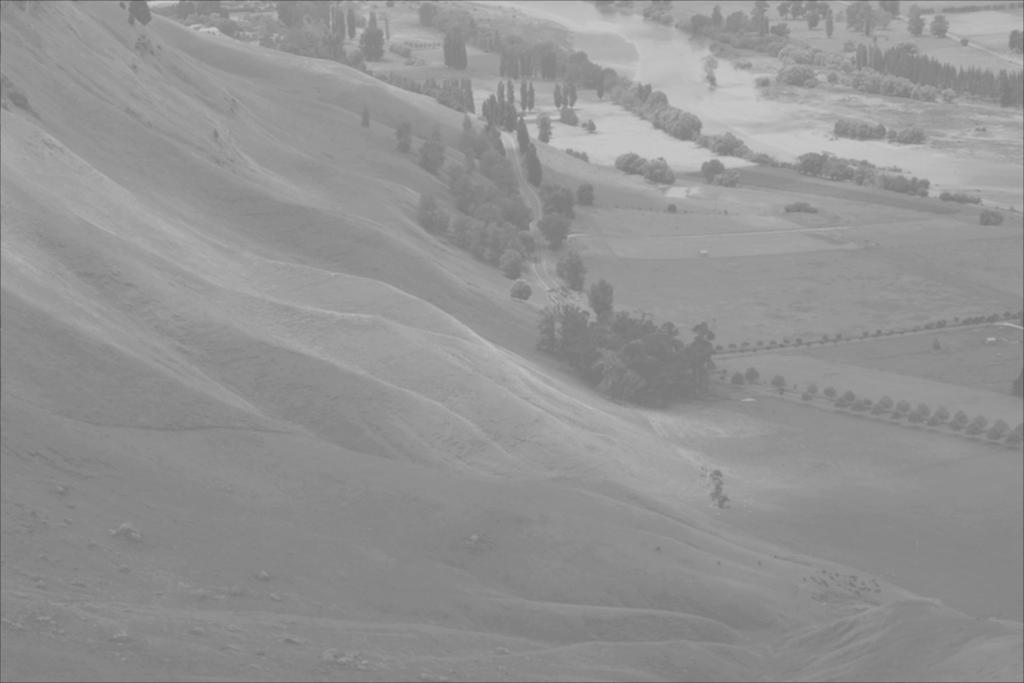
\includegraphics[scale=0.2]{imagens/hawkes-blur.jpg}\\
			\hline
			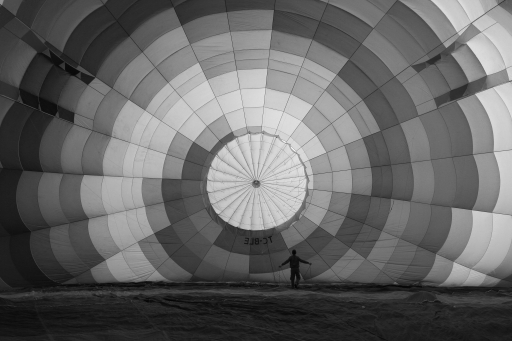
\includegraphics[scale=0.4]{imagens/baloon.JPG}&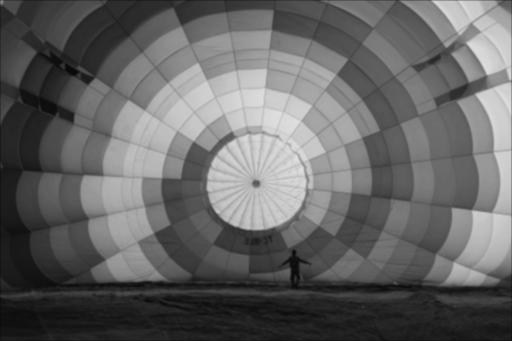
\includegraphics[scale=0.4]{imagens/baloon-blur.jpg}\\
			\hline
			\end{tabular}
			\label{tab:gt}
			\end{table}


	%No método de aumento de nitidez, apresente também a imagem intermediária resultante da aplicação do operador Laplaciano.
	\section{Filtro de Aumento de Nitizez - Sharpening}
		Este filtro visa aumentar a nitidez, ou seja, tornar bordas e detalhes da imagem mais visíveis que anteriormente. Uma imagem candidata a ter este filtro aplicado pode ser alguma que passou anteriormente por um processo de suavização como o que foi detalhado antes ou então alguma em que a captura tenha gerado algum borramento (Uma mão trêmula no momento da captura da imagem, por exemplo). Novamente, esta transformação é linear, sendo o resultado da aplicação do operador Laplaciano. Conforme apresentado no EP, tal operador pode ser descrito através do \emph{8 neighbor Laplacian}, um kernel da forma
\[
 \begin{pmatrix}
  -1 & -1 & -1 \\
  -1 & 8 & -1 \\
  -1 & -1 & -1 \\
 \end{pmatrix}
\]		

		Notamos que o resultado da aplicação desta filtragem por convolução gera uma matriz de diferenças da imagem original para a com a nitidez aumentada. O resultado final pode ser atingido de duas maneiras: Substituindo o coeficiente 8 por nove no kernel ou somar a imagem ao resultado da convolução. 
		
		\subsection{Vantagens e desvantagens}
			Outra vez, uma vantagem deste método é a simplicidade de implementação uma vez que haja como aplicar uma filtragem por convolução. A complexidade é novamente polinomial, cada pixel da imagem filtrada necessida de 9 multiplicações para ser gerada. Porém, este filtro não é tão eficiente quanto outros para o mesmo propósito pois não incorpora nenhum conhecimento prévio das características da imagem, não levando propriedades da figura em consideração que poderiam produzir um resultado melhor.
			
		\subsection{Implementação}
			Utilizando a implementação da filtragem por convolução, o filtro é implementado da seguinte forma:
			
			\begin{lstlisting}
			function [final] = aumentar_nitidez(imagem)
				convolucao = aplicar_convolucao(imagem, [-1 -1 -1; -1 8 -1; -1 -1 -1]);
			    final = imagem + convolucao;
			endfunction
			\end{lstlisting}
			
			\texttt{convolucao} é a matriz de diferenças descrita antes, sendo o resultado da aplicação do operador Laplaciano.
		
		\subsection{Testes realizados}
			Apresentamos além das imagens originais e filtradas também a matriz \texttt{convolucao}, intermediária resultante da aplicação do operador Laplaciano. Notamos que o filtro torna as imagens claramente mais nítidas, prova de sua eficácia.
			\begin{table}[ht]
			\caption{Imagens antes, intermediária e depois de aplicada a filtragem de aumento de nitidez}
			\centering
			\begin{tabular}{|c|c|c|}
			\hline
			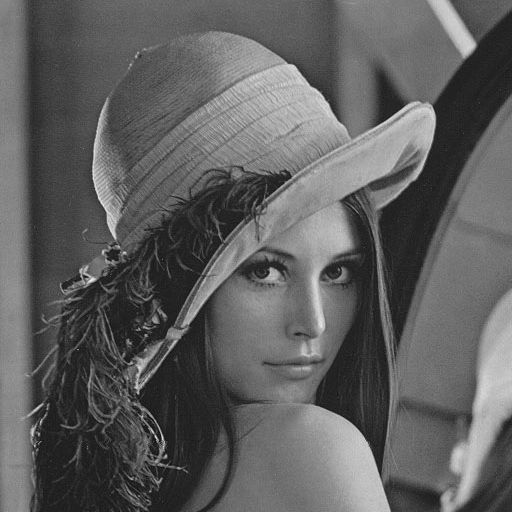
\includegraphics[scale=0.27]{imagens/lena.jpg}&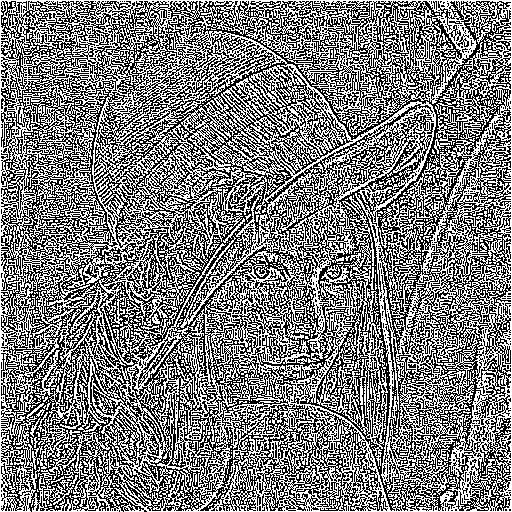
\includegraphics[scale=0.27]{imagens/lena-convolucao.jpg}&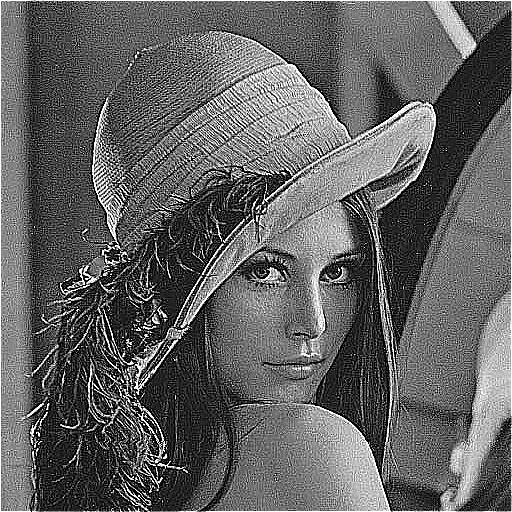
\includegraphics[scale=0.27]{imagens/lena-sharpen.jpg}\\
			\hline
			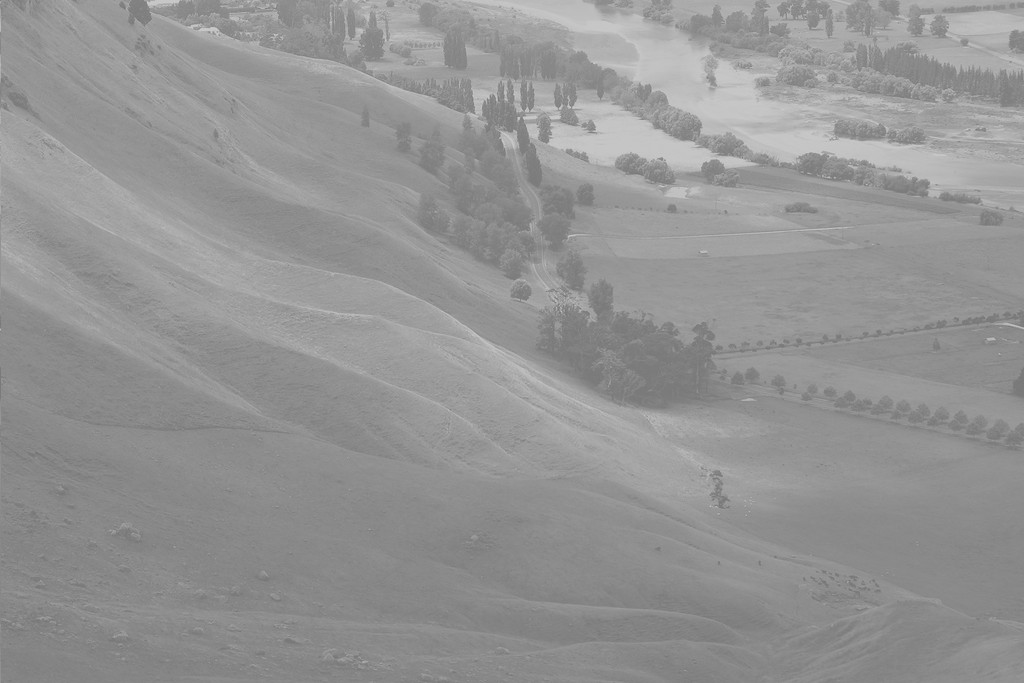
\includegraphics[scale=0.135]{imagens/hawkes.jpg}&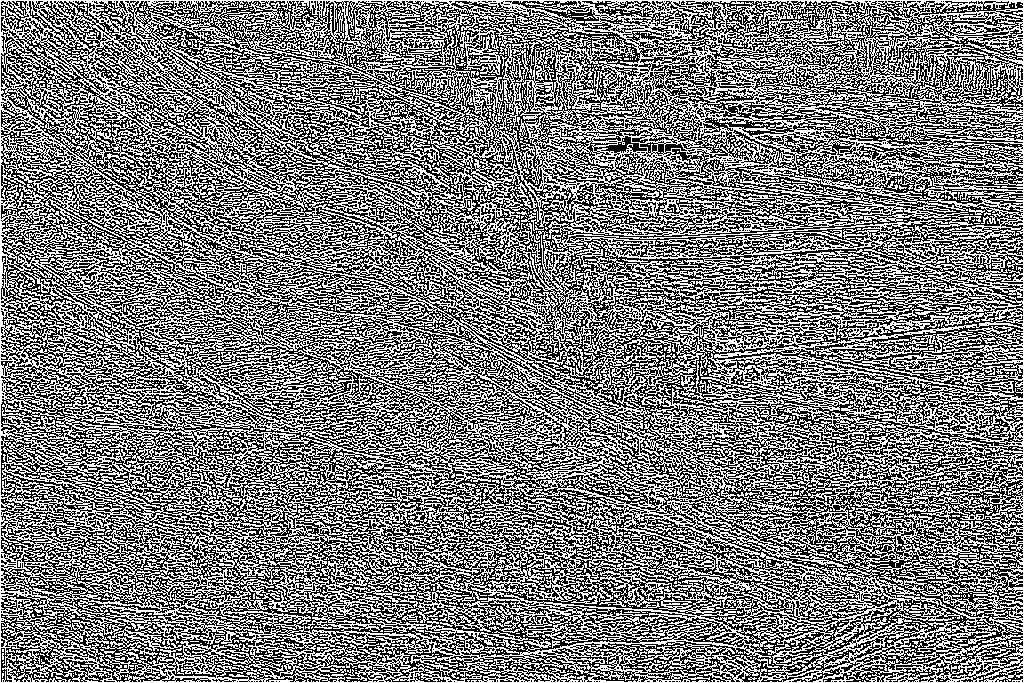
\includegraphics[scale=0.135]{imagens/hawkes-convolucao.jpg}&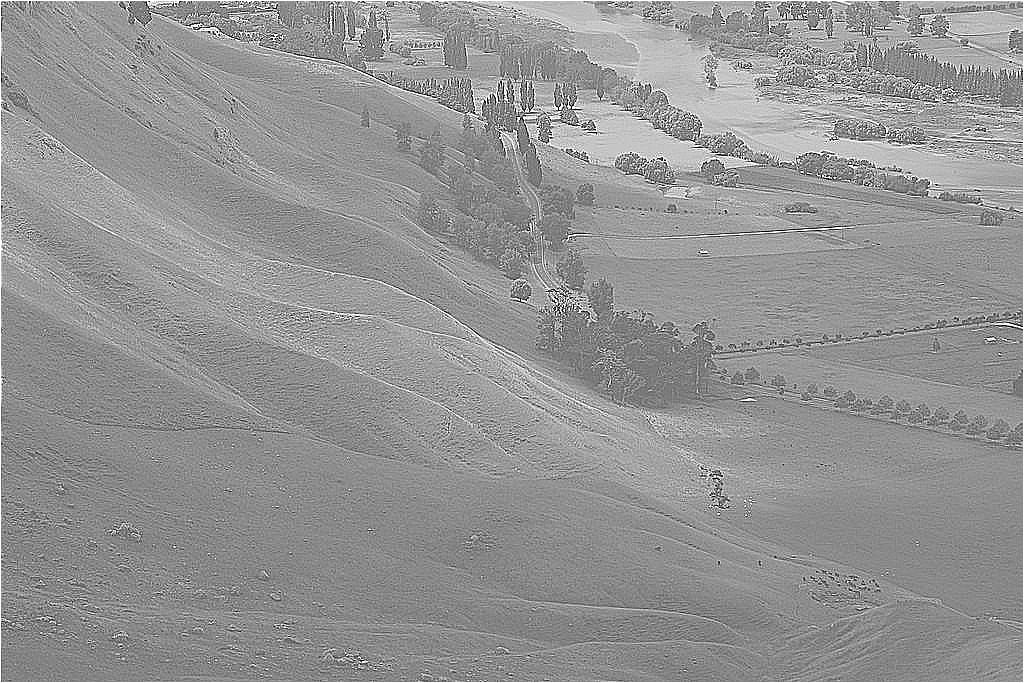
\includegraphics[scale=0.135]{imagens/hawkes-sharpen.jpg}\\
			\hline
			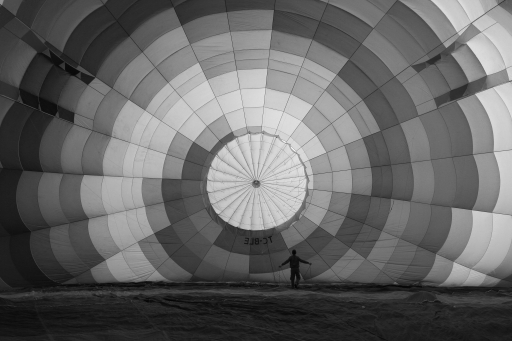
\includegraphics[scale=0.27]{imagens/baloon.JPG}&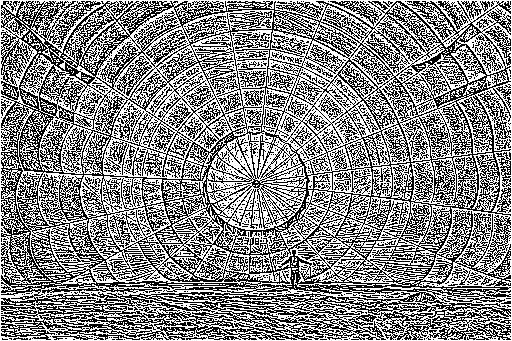
\includegraphics[scale=0.27]{imagens/baloon-convolucao.jpg}&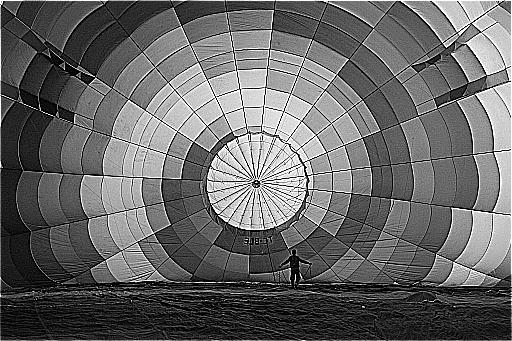
\includegraphics[scale=0.27]{imagens/baloon-sharpen.jpg}\\
			\hline
			\end{tabular}
			\label{tab:gt}
			\end{table}



\chapter{Conclusão}
	O trabalho ajudou os alunos a entrar em contato com a área de Computação Gráfica, pouco abordada durante a os estudos habituais de um aluno de Ciência da Computação. Com uma introdução teórica suficiente e exercícios práticos de implementação relacionados ao assunto os alunos conseguiram fixar os novos conceitos tais como convolução e diferentes métodos de filtragem de imagens. O tema gera mais interesse ainda pela sua conotação visual inerente, que torna mais palatável os resultados obtidos depois dos diversos processamentos.
	
	Novamente, a possibilidade de utilizar uma linguagem voltada pra processamentos matemáticos, tal como Octave, a escolhida para este trabalho, simplificou problemas de implementação, permitindo aos alunos focarem nos algoritmos propriamente ditos. Ainda, a carga de teoria embutida no EP2 diminuiu com relação ao EP1, algo interessante dadas as dificuldades que os alunos enfrentaram ao iniciarem seus trabalhos no EP1.
	
%\nocite{*}
%\bibliographystyle{abnt-num}
%\bibliography{bibliografia}
\end{document}

\end{document}
